%%%%%%%%%%%%%%%%%%%%%%%%%%%%%%%%%%%%%%%%%%%%%%%%%%%
% Signal Processing Laboratory (LTS5) - EPFL      %
% LaTeX student report template                   %
% Authors:                                        %
%   D. Perdios – dimitris.perdios@epfl.ch         %
%   A. Besson – adrien.besson@epfl.ch             %
% v0.1 - 22.12.16                                 %
% Typeset configuration: pdfLaTeX + Biber         %
%%%%%%%%%%%%%%%%%%%%%%%%%%%%%%%%%%%%%%%%%%%%%%%%%%%


%%% DOCUMENT CLASS
%\documentclass[10pt,a4paper,twoside,openright]{lts5student}
\documentclass[10pt,a4paper,oneside]{lts5student}

%%% PACKAGES DECLARATION
%%%%%%%%%%%%%%%%%%%%%%%%%%%%%%%%%%%%%%%%%%%%%%%%%%%
% Signal Processing Laboratory (LTS5) - EPFL      %
% LaTeX student report template                   %
% Authors:                                        %
%   D. Perdios – dimitris.perdios@epfl.ch         %
%   A. Besson – adrien.besson@epfl.ch             %
% v0.1 - 22.12.16                                 %
% Typeset configuration: pdfLaTeX + Biber         %
%%%%%%%%%%%%%%%%%%%%%%%%%%%%%%%%%%%%%%%%%%%%%%%%%%%


% Document layout
%\usepackage[showframe=true,pass=true]{geometry} % Useful to check the document margin layout

% Typesetting
\usepackage[T1]{fontenc}
\usepackage[utf8]{inputenc}
\usepackage[english]{babel}
\usepackage{lmodern} % latin modern font
\usepackage[scaled]{helvet} % sans serif typo
\usepackage{csquotes} % pro­vides ad­vanced fa­cil­i­ties for in­line and dis­play quo­ta­tions (better to load when using biblatex)
\usepackage{textcomp} % pro­vide many text sym­bols (such as baht, bul­let, copy­right, mu­si­cal­note, onequar­ter, sec­tion, and yen), in the TS1 en­cod­ing
%\usepackage{setspace}
%	\onehalfspacing % 1.5 linespaceing (already in CLS)
%\usepackage{fancyhdr} % pro­vides ex­ten­sive fa­cil­i­ties, both for con­struct­ing head­ers and foot­ers, and for con­trol­ling their use
\usepackage{siunitx}
\sisetup{
	group-digits = integer, % only group digits (by three) for integers (not decimals)
	binary-units = true, % load binary units
	detect-all
} % SI units system typset
%\usepackage{enumitem}
%	\setlist[enumerate]{label*=\arabic*.,topsep=5pt,partopsep=0pt,parsep=0pt,itemsep=2pt}
%	\setlist[itemize]{topsep=5pt,partopsep=0pt,parsep=0pt,itemsep=2pt}
\usepackage{bigfoot} % The pack­age aims to pro­vide a 'one-stop' so­lu­tion to re­quire­ments for foot­notes
\usepackage{afterpage} % to use \footnotemark and \footnotetext in captions for special cases
\usepackage{algorithm} % the al­go­rithm pack­age de­fines a float­ing al­go­rithm en­vi­ron­ment de­signed to work with the al­go­rith­mic style
\usepackage{algpseudocode} % The algorithmicx package provides many possibilities to customize the layout of algorithms.

% Math
\usepackage{amsmath}
\usepackage{amsfonts}
\usepackage{amssymb}
\usepackage{amsthm}
\usepackage{bm}

% Figures
\usepackage{graphicx} % [draft] option usefull
	\graphicspath{{figures/}}
\usepackage{xcolor}
%\usepackage[font=small, labelfont=bf, format=plain, labelsep=space, figurename=Figure, tablename=Table, skip=5pt]{caption} % defined in CLS
\usepackage[labelfont=rm, labelformat=parens, labelsep=space, skip=0pt]{subcaption} % defined in CLS

% Tables
\usepackage{multirow}
\usepackage{longtable} % use \linebreak instead of \\ in headers to avoid a bug with longtables (or longtabu) across two pages
\usepackage{booktabs} % the pack­age en­hances the qual­ity of ta­bles (toprule, bottomrule, etc.)
\usepackage{tabu}
	\renewcommand{\arraystretch}{1.3}

% Others
%\usepackage[draft]{pdfpages} % include pdf pages
\usepackage{calc}
%\usepackage{todonotes} % \todo, \missingfigures and \listoftodos
\usepackage{xifthen} % This pack­age ex­tends the ifthen pack­age by im­ple­ment­ing new com­mands to go within the first ar­gu­ment of \ifthenelse
\usepackage{lipsum} % Lorem Ip­sum dummy text
	\newcommand{\mylipsum}[1][]{\ifthenelse{\isempty{#1}}{\textcolor{gray}{\lipsum}}{\textcolor{gray}{\lipsum[#1]}}}
\usepackage{blindtext} % Pro­vides the com­mands \blind­text and \Blind­text for cre­at­ing ‘blind’ text use­ful in test­ing new classes and pack­ages, and \blind­doc­u­ment, \Blind­doc­u­ment for cre­at­ing an en­tire ran­dom doc­u­ment with sec­tions, lists, math­e­mat­ics, etc.

% Biblatex
\usepackage[backend=biber,bibstyle=ieee,citestyle=ieee]{biblatex} % style=ieee loads both, bibstyle and citestyle

% References and urls
\usepackage{url}
%\usepackage[pdfusetitle]{hyperref} 	% pdfusetitle = author and title used for pdf name
\usepackage{hyperref}
	\hypersetup{
%		hypertexnames=false,			% hypertexnames option only used with autnum packages
%		bookmarks=true,         		% show bookmarks bar?
		bookmarksnumbered=true,		% section numbers in pdf bookmarks
%    	unicode=false,				% non-Latin characters in Acrobat’s bookmarks
%    	pdftoolbar=true,				% show Acrobat’s toolbar?
%    	pdfmenubar=true,				% show Acrobat’s menu?
%    	pdffitwindow=false,			% window fit to page when opened
%    	pdfstartview={FitH},			% fits the width of the page to the window
%		pdftitle={\runauthor{} - \runtitle{}}, % title
%		pdfauthor={\runauthor{}},	% author
%    	pdfsubject={Subject},		% subject of the document
%    	pdfcreator={Creator},		% creator of the document
%    	pdfproducer={Producer},		% producer of the document
%    	pdfkeywords={keyword1, key2, key3}, % list of keywords
%    	pdfnewwindow=true,			% links in new PDF window
		colorlinks=true, 			% false: boxed links; true: colored links
		pdfborder={0 0 0},			% box border style
		linkcolor=black,				% color of internal links (change box color with linkbordercolor)
		citecolor=black,				% color of links to bibliography
		filecolor=black,				% color of file links
		urlcolor=black				% color of external links
	}
\usepackage{bookmark} % Im­ple­ments a new book­mark (out­line) or­ga­ni­za­tion for pack­age hy­per­ref
%TODO: if bookmark and hyperref not loaded, \phantomsection and \pdfbookmark won't be defined
%\providecommand\phantomsection{}	% in case hyperref or bookmark is not loaded it allows \phatomsection
%\usepackage{cleveref}				% MUST be loaded after hyperref
%%%%%%%%%%%%%%%%%%%%%%%%%%%%%%%%%%%%%%%%%%%%%%%%%%%
% Signal Processing Laboratory (LTS5) - EPFL      %
% LaTeX student report template                   %
% Authors:                                        %
%   D. Perdios – dimitris.perdios@epfl.ch         %
%   A. Besson – adrien.besson@epfl.ch             %
% v0.1 - 22.12.16                                 %
% Typeset configuration: pdfLaTeX + Biber         %
%%%%%%%%%%%%%%%%%%%%%%%%%%%%%%%%%%%%%%%%%%%%%%%%%%%


% Useful to include specific packages

%%% TITLE & AUTHORS SETTINGS
\title{Gender recognition by voice}
\author{Adrien Besson}
\authortwo{Hippolyte Lefebvre}
\authorthree{Greg}
\supervisor{Dr. Emeric Thibaud}
\projecttype{Project}
\date{\today}

%%% BIBLIOGRAPHY
% 	Settings
%%%%%%%%%%%%%%%%%%%%%%%%%%%%%%%%%%%%%%%%%%%%%%%%%%%
% Signal Processing Laboratory (LTS5) - EPFL      %
% LaTeX student report template                   %
% Authors:                                        %
%   D. Perdios – dimitris.perdios@epfl.ch         %
%   A. Besson – adrien.besson@epfl.ch             %
% v0.1 - 22.12.16                                 %
% Typeset configuration: pdfLaTeX + Biber         %
%%%%%%%%%%%%%%%%%%%%%%%%%%%%%%%%%%%%%%%%%%%%%%%%%%%


% Known problems with biblatex-ieee style
% 1) still problems with arXiv (eprint) having a primaryClass (eprintclass) entry. The output is ok, i.e. arXiv: <eprint> [<primaryClass>], but the href is not correct and does not include the <primaryClass>. For exemple it would link to http://arxiv.org/abs/407151 instead of http://arxiv.org/abs/astro-ph/407151 (<arxiv>=40751, <primaryClass>=astro-ph).
%	Maybe a problem due to Mendeley export which should export <arxiv>=40751/astro-ph without any <primaryClass> field
% 2) if more than one url is given it seems not to be a list an adds %20 (space char) between each links...

%% LOAD OPTIONS
% 	Remark 1: backend, style, bibstyle and citestyle options as well natbib and mcite compatibility options must be set at loading time in the square brackets
%	Remark 2: \ExecuteBibliographyOptions[<entrytype, ...>]{<key=value, ...>} 
%	Remark 3: seems better than clearfield since it doesn't clear the field, just doesn't print
%\ExecuteBibliographyOptions{citestyle=numeric-comp} % nicer than the ieee citestyle
%\ExecuteBibliographyOptions{sorting=none} % sorting=none already defined by ieee
\ExecuteBibliographyOptions{mincitenames=3} % if more than maxcitename, truncates to mincitename
\ExecuteBibliographyOptions{maxcitenames=3} % if more than maxcitename, truncates to mincitename
\ExecuteBibliographyOptions{minbibnames=6} % if more than maxbibname, truncates to minbibname
\ExecuteBibliographyOptions{maxbibnames=6} % if more than maxbibname, truncates to minbibname
%\ExecuteBibliographyOptions{isbn=false}
%\ExecuteBibliographyOptions{doi=false}
%\ExecuteBibliographyOptions{eprint=false}
%\ExecuteBibliographyOptions{url=false} % does not affect @online since url is mandatory 
%\ExecuteBibliographyOptions{firstinits=true} % already defined by ieee bibstyle
%\ExecuteBibliographyOptions{date=year}

%% SOME BASIC CUSTOMIZATIONs
% 	Bilbiography font size
%\renewcommand*{\bibfont}{\small}

% 	Bibliography item separation
%\setlength\bibitemsep{0pt}		% No separation between bib entries

% 	Bibliography name
%TODO: change bibliography name in the .cls file by using \refname instead of \bibname for the chapter name

% At every bibitem
%TODO: how not to print an entry without clearing it
\AtEveryBibitem{% Clean up the bibtex rather than editing it
% 	\clearlist{address}
%	\clearfield{abstract}
%	\clearfield{title}
%	\clearname{author}
% 	\clearfield{date}
 	\clearfield{doi}
% 	\clearfield{eprint}
 	\clearfield{isbn}
 	\clearfield{issn}
 	\clearfield{isrn}
% 	\clearlist{location}
 	\clearfield{month}
 	\clearfield{number}
%	\clearfield{note}
%	\clearfield{url}
%	\clearfield{issue}
 	\clearfield{series}
% 	\clearname{editor}
 	
 	% Remove arXiv (eprint) for @article if journaltitle (which is converted from .bib journal entry) exists
 	\ifentrytype{article}
 		{
 			\iffieldundef{journaltitle}
 				{}
 				{\clearfield{eprint}}
 		}
 		{}
 	% Remove arXiv (eprint) for @inproceedings if booktitle exists
	\ifentrytype{inproceedings}
 		{
 			\iffieldundef{booktitle}
 				{}
 				{\clearfield{eprint}}
 		}
 		{}
	% Remove publisher, location and editor except for @book
 	\ifentrytype{book}
 		{}
 		{
  			\clearlist{publisher}
  			\clearlist{location}
  			\clearname{editor}
		}
	% Remove url except for @online (similar to using url=false package option)
	\ifentrytype{online}
 		{}
 		{\clearfield{url}}
}

% At every citekey
%TODO: check \AtEveryCitekey
%\AtEveryCitekey{
%	\clearfield{month}
%}

% Preserve acronyms in titles which are lowcased by ieee style
%	Remark 1: the expression \b\w*[A-Z]{2,}\w*\b finds a word containing at least 2 capital letters
%	Remark 2: (expr) group elements of the expression and capture tokens
%	Remark 3: replace expr wrapping it in curly braces (don't know why the empty group is needed, see http://tex.stackexchange.com/questions/238078/biblatex-preserve-case-of-acronyms-in-title)
%	Remark 4: changing [A-Z]{2,} to [A-Z]{1,} would preserve the uppercase of every words
%TODO: check with 2016 version of TeX and new versions of biblatex-ieee yet freezed
\DeclareSourcemap{
	\maps[datatype=bibtex]{
		\map{
			\step[fieldsource=title, match=\regexp{(\b\w*[A-Z]{2,}\w*\b)}, replace={{}{$1}}]
		}
	}
}

% More intelligent initials, for exemple, Ph. for Philippe rather than P. (see: http://tex.stackexchange.com/questions/295476/two-or-three-letter-initials-in-bibliography-with-biblatex)
\DeclareStyleSourcemap{%
	\maps[datatype=bibtex]{%
	\map{%
		% Author field
		\step[fieldsource=author,%
			match={\regexp{\b(Chr|Ch|Th|Ph|[B-DF-HJ-NP-TV-XZ](l|r))(\S*,)}},%
			replace={\regexp{\{$1\}$3}}]% Protect last names (first last)
		\step[fieldsource=author,%
			match={\regexp{([^,]\s)\b(Chr|Ch|Th|Ph|[B-DF-HJ-NP-TV-XZ](l|r))}},%
			replace={\regexp{$1\{$2\}}}]% Protect last names (last, first)
		\step[fieldsource=author,%
			match={\regexp{\b(Chr|Ch|Th|Ph|[B-DF-HJ-NP-TV-XZ](l|r))([^\}])}},%
			replace={\regexp{\{\\relax\{\}$1\}$3}}]% Insert \relax after abbreviating
		% Editor field
		\step[fieldsource=editor,%
			match={\regexp{\b(Chr|Ch|Th|Ph|[B-DF-HJ-NP-TV-XZ](l|r))(\S*,)}},%
			replace={\regexp{\{$1\}$3}}]% Protect last names (first last)
		\step[fieldsource=editor,%
			match={\regexp{([^,]\s)\b(Chr|Ch|Th|Ph|[B-DF-HJ-NP-TV-XZ](l|r))}},%
			replace={\regexp{$1\{$2\}}}]% Protect last names (last, first)
		\step[fieldsource=editor,%
			match={\regexp{\b(Chr|Ch|Th|Ph|[B-DF-HJ-NP-TV-XZ](l|r))([^\}])}},%
			replace={\regexp{\{\\relax\{\}$1\}$3}}]% Insert \relax after abbreviating
}}}%


% Typeset only the first page with p. instead of pp. for any entry
%\DeclareFieldFormat{pages}{\mkfirstpage[{\mkpageprefix[bookpagination]}]{#1}}

% Make volume typset bold
%\DeclareFieldFormat[article,periodical]{volume}{\mkbibbold{#1}}

% Removing the in
% 		for every entries
%\renewbibmacro{in:}{}
%% 		only for articles
%\renewbibmacro{in:}{%
%  \ifentrytype{article}{}{\printtext{\bibstring{in}\intitlepunct}}}

% 	Bibliography resources
\addbibresource{project_bib.bib} % Input bibliography file

%%% HEADERS SETTINGS
\pagestyle{headings}

%%% NEWCOMMANDS
%%%%%%%%%%%%%%%%%%%%%%%%%%%%%%%%%%%%%%%%%%%%%%%%%%%
% Signal Processing Laboratory (LTS5) - EPFL      %
% LaTeX student report template                   %
% Authors:                                        %
%   D. Perdios – dimitris.perdios@epfl.ch         %
%   A. Besson – adrien.besson@epfl.ch             %
% v0.1 - 22.12.16                                 %
% Typeset configuration: pdfLaTeX + Biber         %
%%%%%%%%%%%%%%%%%%%%%%%%%%%%%%%%%%%%%%%%%%%%%%%%%%%


% Useful to create specific newcommands
\newcommand{\ie}{\textit{i.e.}}
\newcommand{\eg}{\textit{e.g.}}

% Tables spacing
\newcommand{\ra}[1]{\renewcommand{\arraystretch}{#1}}

% Math
\newcommand*{\abs}[1][]{\left\lvert#1\right\rVert}
\newcommand*{\norm}[2][]{\left\lVert#2\right\rVert_{#1}}
\newcommand*{\zeronorm}[1]{\norm[0]{#1}}
\newcommand*{\onenorm}[1]{\norm[1]{#1}}
\newcommand*{\twonorm}[1]{\norm[2]{#1}}
\newcommand*{\twoonenorm}[1]{\norm[2,1]{#1}}
\newcommand*{\fronorm}[1]{\norm[F]{#1}}
\newcommand*{\infnorm}[1]{\norm[\infty]{#1}}
\newcommand*{\pnorm}[1]{\norm[p]{#1}}
\newcommand*{\tvnorm}[1]{\norm[TV]{#1}}
\newcommand*{\mat}[1]{\mathbf{#1}}

% Sets
\newcommand*{\C}{\mathbb{C}}
\newcommand*{\R}{\mathbb{R}}
\newcommand*{\Q}{\mathbb{Q}}
\newcommand*{\Z}{\mathbb{Z}}

%%% BEGIN DOCUMENT
\begin{document}

%%%%%%%%%%%%%%%%%%%%%%%%%%%%%%%%%%%%%%%%%%%%%%
%%%%% HEAD: Title, ToC, ToF, ...
%%%%%%%%%%%%%%%%%%%%%%%%%%%%%%%%%%%%%%%%%%%%%%
%%%%%%%%%%%%%%%%%%%%%%%%%%%%%%%%%%%%%%%%%%%%%%%%%%%
% Signal Processing Laboratory (LTS5) - EPFL      %
% LaTeX student report template                   %
% Authors:                                        %
%   D. Perdios – dimitris.perdios@epfl.ch         %
%   A. Besson – adrien.besson@epfl.ch             %
% v0.1 - 22.12.16                                 %
% Typeset configuration: pdfLaTeX + Biber         %
%%%%%%%%%%%%%%%%%%%%%%%%%%%%%%%%%%%%%%%%%%%%%%%%%%%


\maketitle
\cleardoublepage\phantomsection
\pdfbookmark[chapter]{\contentsname}{toc}
\tableofcontents
\cleardoublepage\phantomsection
\addcontentsline{toc}{chapter}{\listfigurename}
\listoffigures
\cleardoublepage\phantomsection
\addcontentsline{toc}{chapter}{\listtablename}
\listoftables
\cleardoublepage\phantomsection
%TODO: check if a list is empty before printing it (see: http://tex.stackexchange.com/questions/113769/add-list-of-figures-tables-only-when-content)

%%%%%%%%%%%%%%%%%%%%%%%%%%%%%%%%%%%%%%%%%%%%%%
%%%%% MAIN: The chapters of the thesis
%%%%%%%%%%%%%%%%%%%%%%%%%%%%%%%%%%%%%%%%%%%%%%
%%%%%%%%%%%%%%%%%%%%%%%%%%%%%%%%%%%%%%%%%%%%%%%%%%%
% Signal Processing Laboratory (LTS5) - EPFL      %
% LaTeX student report template                   %
% Authors:                                        %
%   D. Perdios – dimitris.perdios@epfl.ch         %
%   A. Besson – adrien.besson@epfl.ch             %
% v0.1 - 22.12.16                                 %
% Typeset configuration: pdfLaTeX + Biber         %
%%%%%%%%%%%%%%%%%%%%%%%%%%%%%%%%%%%%%%%%%%%%%%%%%%%


\chapter{Introduction}
\label{chap:introduction}

In the last decades, automatic gender recognition~(AGR) from speech has grown many interest thanks to the digitization of an extensive number of applications and the development of mobile platforms~\cite{Wu_JASA_1991, Wu_JASA_1991_2, Childers_ICASSP_1988, Harb2005, Zeng2006, Sorokin2008, Metze_ICASSP_2007, Bocklet_ICASSP_2008}.

The applications of AGR have increased consequently. Indeed, in general, the accuracy of gender-dependent systems is higher than the one of gender-independent systems~\cite{Harb2005}. Thus, AGR improves the prediction of other speaker traits such as age~\cite{Levi2015} and emotional state~\cite{Bisio2013, Ververidis2004}. It can also facilitate speech recognition by gender-based normalization~\cite{Wegmann_ICASSP_1996} and is a key feature for more natural and personalized dialog systems such as Siri.

The AGR techniques are based on statistical features extracted from the speech signals such as maximum, minimum and average frequency measured in a time span. These features translate physiological differences between males and females like the length of the vocal chords or the glottal shape~\cite{Titze_JASA_1989}. Among all the features, it appears that the fundamental frequency plays a crucial role in gender classification as described in many studies~\cite{Hollien1967, Wu_JASA_1991, Poon2015}. In recent works, the use of the fundamental frequency coupled with spectral components such as Mel-frequency spectral components~\cite{Gupta2016} or relative spectral perceptual linear predictive coefficients~\cite{Zeng2006} have demonstrated best AGR performances even in noisy environments.

In this project, we study different state-of-the-art classification methods applied to the task of gender recognition by voice. The study is based on a dataset of features extracted from \num{3168} subjects available on Kaggle\footnote{\url{https://www.kaggle.com/primaryobjects/voicegender}} and described in details in Chapter~\ref{chap:dataset}. A preliminary exploratory data analysis is performed in Chapter~\ref{chapter_data_exploration} which gives many hints for the evaluation of the classification methods, described in Chapter~\ref{chapter_classification}. Eventually, the best classification model is tested on \num{11} voices recorded by the authors in Chapter~\ref{chap_test_our_dataset}.
  
%%%%%%%%%%%%%%%%%%%%%%%%%%%%%%%%%%%%%%%%%%%%%%%%%%%
% Signal Processing Laboratory (LTS5) - EPFL      %
% LaTeX student report template                   %
% Authors:                                        %
%   D. Perdios – dimitris.perdios@epfl.ch         %
%   A. Besson – adrien.besson@epfl.ch             %
% v0.1 - 22.12.16                                 %
% Typeset configuration: pdfLaTeX + Biber         %
%%%%%%%%%%%%%%%%%%%%%%%%%%%%%%%%%%%%%%%%%%%%%%%%%%%

\chapter{Description of the Dataset}
\label{chap:dataset}

\section{General considerations}
\label{sec:gen_cons}
The voice gender dataset\footnote{\url{https://www.kaggle.com/primaryobjects/voicegender}} consists of features extracted from \num{3168} recorded voice samples, collected from male and female speakers. 
The features have been extracted from the voice recordings using tuneR\footnote{\url{https://cran.r-project.org/web/packages/tuneR/tuneR.pdf}} and seewave\footnote{\url{https://cran.r-project.org/web/packages/seewave/seewave.pdf}}, two acoustic analysis packages of R.

The dataset takes the form of a ``.csv'' file where each row is composed of the following acoustical features:
\begin{itemize}
	\item \textbf{meanfreq:} mean frequency (in kHz)
	\item \textbf{sd:} standard deviation of frequency
	\item \textbf{median:} median frequency (in kHz)
	\item \textbf{Q25:} first quantile (in kHz)
	\item \textbf{Q75:} third quantile (in kHz)
	\item \textbf{IQR:} interquantile range (in kHz)
	\item \textbf{skew:} skewness of the spectrum
	\item \textbf{kurt:} kurtosis
	\item \textbf{sp.ent:} spectral entropy
	\item \textbf{sfm:} spectral flatness
	\item \textbf{mode:} mode frequency
	\item \textbf{centroid:} frequency centroid 
	\item \textbf{peakf:} peak frequency (frequency with highest energy)
	\item \textbf{meanfun:} average of fundamental frequency measured across acoustic signal
	\item \textbf{minfun:} minimum fundamental frequency measured across acoustic signal
	\item \textbf{maxfun:} maximum fundamental frequency measured across acoustic signal
	\item \textbf{meandom:} average of dominant frequency measured across acoustic signal
	\item \textbf{mindom:} minimum of dominant frequency measured across acoustic signal
	\item \textbf{maxdom:} maximum of dominant frequency measured across acoustic signal
	\item \textbf{dfrange:} range of dominant frequency measured across acoustic signal
	\item \textbf{modindx:} modulation index. Calculated as the accumulated absolute difference between adjacent measurements of fundamental frequencies divided by the frequency range
	\item \textbf{label:} male or female
\end{itemize}

The features are all quantitative and represent frequency characteristics of the voices.
\section{Description of the features}
\label{sec:feat_desc}
Before starting the data analysis, it is important to perfectly understand the features involved in the exercise. This will be very useful in a preprocessing step, since it will allow us to remove collinear features. It will also be a great asset when it will come to the analysis of the most important features involved in the classification process.

As already pointed out in Section~\ref{sec:gen_cons}, the extracted features are all related to the spectrum. 
\paragraph{Frequency-related features}
The feature ``meanfun'' corresponds to  the mean frequency, \ie{} a weighted average of the frequencies present in the spectrum by the amplitude of the spectral components:
\begin{equation}
\mu_f = \sum\limits_{i=1}^{N} f_i y_i ,
\end{equation} 
where $N$ is the number of frequency components of the spectrum, $f_i$ is the i-th frequency and $y_i$ is the relative amplitude of the i-th component of the spectrum. 
As described p.\num{163} of the seewave documentation, it is equal to the feature ``centroid''.
The feature ``sd'' is the standard deviation of the frequencies, calculated as:
\begin{equation}
\sigma_f = \sqrt{\sum\limits_{i=1}^{N}y_i \left(f_i-\ie\mu_f\right)^2}.
\end{equation}

The feature ``median'' is the median frequency calculated as the frequency where the spectrum is divided into frequency intervals of same energy. The calculation of the quartiles ``IQ25'' and  ``IQ75'' is based on the same criterion. The interquartile range ``IQR'' is calculated as the difference between the first and the first quartile.

The feature ``mode'' characterizes the dominant frequency of the spectrum, \ie{} the frequency with the highest amplitude. It is very similar to ``peakf'', the peak frequency, which corresponds to the frequency with the highest energy. The fundamental frequency is the lowest frequency of the spectrum.

The features ``meanfun'', ``minfun'', ``maxfun'', ``meandom'', ``maxdom'', ``mindom'', ``dfrange'' and ``modindx'' are calculated as the mean, minimum and maximum values of the fundamental and dominant frequencies respectively, where the mean, maximum and minimum are taken across many time segments which compose a given voice recording.

In addition to the frequency-related features, we can find measures on the shape of the spectrum which may give very interesting additional information. 
\paragraph{Skewness of the spectrum}
The skewness of the spectrum is a measure of its asymmetry around the mean frequency. It is calculated as follows:
\begin{equation}
\label{eq_skew}
	S = \frac{1}{\sigma_f^3}\frac{\sum\limits_{i=1}^{N} \left(f_i - \mu_f\right)^3}{N-1}.
\end{equation}
From~\eqref{eq_skew}, it is clear that the sign of $S$ gives information of the left or right asymmetry of the spectrum while the absolute value of $S$ gives the strength of the asymmetry. 
\paragraph{Kurtosis}
The kurtosis is a measure of the ``tailedness'' of a probability distribution. It is calculated as the fourth order moment of the frequency distribution, described below:
\begin{equation}
\label{eq_kurtosis}
	K = \frac{1}{\sigma_f^4}\frac{\sum\limits_{i=1}^{N} \left(f_i - \mu_f\right)^4}{N-1}.
\end{equation}
When $K=3$, the frequency distribution is normal. When $K<3$, the frequency distribution is said to be \textit{platikurtic}, it has fewer items around the means than in the tails, compared to a normal distribution. When $K>3$, the distribution is said to be \textit{leptokurtic} and has more frequency around the mean than in the tails, compared to a normal distribution.
\paragraph{Shannon spectral entropy}
The Shannon entropy is used to discriminate whether the voice signal is noisy or pure~\cite{Nunes2004}. It is calculated as follows:
\begin{equation}
\label{eq:entropy}
	H = \frac{-\sum\limits_{i=1}^{N} y_i \log_2 \left(y_i\right)}{\log_2 \left(N\right)}.
\end{equation}

If the signal is pure, then all the energy is concentrated in one frequency component, \ie{} $y_i = \delta_{ij}$ and $H=0$. If the signal is a white noise, then $y_i = 1/N, \; \forall i \in \left\lbrace 1,...,N \right\rbrace$ and $H=1$.
\paragraph{Spectral flatness}
The spectral flatness is rather similar to the spectral entropy. It is measured as the ratio between the geometric mean and the arithmetic mean:
\begin{equation}
\label{eq:spec_flat}
	F = N \frac{\sqrt[N]{\prod\limits_{i=1}^{N} y_i}}{\sum \limits_{i=1}^{N} y_i}.
\end{equation}
In case of a white noise, the spectrum is flat and $H=1$. In case of a pure tone, the geometrical mean is equal to zero and $H=0$.

\section{Cleaning the dataset}
\label{sec_cleaning_dataset}
From the description of the features given in Section~\ref{sec:feat_desc}, a first cleaning of the dataset may be achieved before starting the analysis.
Indeed, several features are exactly the same or a linear combination of other features:
\begin{itemize}
	\item The features ``meanfreq'' and ``centroid'' are exactly similar. So ``centroid'' has been removed;
	\item The following relationship holds:  ``IQR'' $=$ ``Q75'' $-$ ``Q25''. ``IQR'' has been removed;
	\item The following relationship holds:  ``dfrange'' $=$ ``maxdom'' $-$ ``mindom''. ``dfrange'' has been removed.
\end{itemize}
\chapter{Exploratory Data Analysis}
\label{chapter_data_exploration}

As a preliminary step, we propose to perform an exploratory data analysis. This will give us some hints about the dataset, \eg the most important features, their correlation etc.

In order to have a first overview of the features, a short description is summarized in Table~\ref{tab_data_exploration}. It can be noticed the frequencies have low values, which makes sense since they are expressed in \si{\kilo\hertz}. 
The mean fundamental frequency is about \SI{143}{\hertz} which is coherent with the male and female fundamental frequencies~\cite{Traunmller1994}. 

Regarding the shape of the spectrum, the mean skewness indicates an average right-asymmetry of the spectrum. The mean kurtosis shows that the frequency distribution is leptokurtic. About the flatness of the spectrum, the features ``sfm'' and ``sp.ent'' seem to have inconsistent behaviour with respect to the their average value since one is above \num{0.5} and the other is below. However, the high standard deviation of ``sfm'' makes an analysis rather difficult.

%%%%%%%%%%%% TABLE %%%%%%%%%%%
\begin{table}[htb]
	\ra{1.2}
	\caption{Description of the features of the dataset}
	 \begin{subtable}{\textwidth}
			\centering
			\begin{tabular}{@{} c c c c  c c c c c c @{}}\toprule
				& meanfreq & sd & median & Q25 & Q75 & skew & kurt & sp.ent & sfm \\
			mean & \num{0.181} &\num{0.0571} & \num{0.186} & \num{0.140} & \num{0.225} & \num{3.14} &\num{36.6} & \num{0.895} &	\num{0.408} \\
			std & \num{0.0299} & \num{0.0167} & \num{0.0364} & \num{0.0487} & \num{0.0236} & \num{4.24} & \num{134} & \num{0.0450} & \num{0.178} \\
			min & \num{0.0394} & \num{0.0184} & \num{0.0110} & \num{0.000229} & \num{0.0429} & \num{0.142} & \num{2.07} & \num{0.739} & \num{0.0369} \\
			\SI{25}{\percent} & \num{0.164} & \num{0.0420} & \num{0.170} & \num{0.111} & \num{0.209} & \num{1.65} & \num{5.67} & \num{0.863} & \num{0.258} \\
			\SI{50}{\percent} & \num{0.185} & \num{0.0592} & \num{0.190} & \num{0.140} & \num{0.226} & \num{2.20} & \num{8.32} & \num{0.902} & \num{0.396} \\
			\SI{75}{\percent} & \num{0.199} & \num{0.0670} & \num{0.211}  & \num{0.176} & \num{0.244} & \num{2.93} & \num{13.7} & \num{0.929} & \num{0.534} \\
			max & \num{0.251} & \num{0.115} & \num{0.261} & \num{0.247} &
			\num{0.273} & \num{34.7} & \num{1310} & \num{0.982} & \num{0.843} \\ \bottomrule
			\end{tabular}
		\end{subtable}\hfill\null%

		\begin{subtable}{\textwidth}
			\centering
			\begin{tabular}{@{} c c c c  c c c c c @{}}\toprule
			 & mode & meanfun & minfun & maxfun & meandom & mindom & maxdom & modindx \\
			mean & \num{0.165} & \num{0.143} & \num{0.0368} & \num{0.259} & \num{0.829} & \num{0.0526} & \num{5.05} & \num{0.174} \\
			std & \num{0.0772} & \num{0.0323} & \num{0.0192} & \num{0.0301} & \num{0.525} & \num{0.0633} & \num{3.52} & \num{0.119} \\
			min & \num{0.00} & \num{0.0556} & \num{0.00977} & \num{0.103} & \num{0.00781} & \num{0.00488} & \num{0.00781} & \num{0.00} \\
			\SI{25}{\percent} & \num{0.118} & \num{0.117} & \num{0.0182} & \num{0.254} & \num{0.420} & \num{0.00781} & \num{2.07} & \num{0.0998} \\
			\SI{50}{\percent} & \num{0.187} & \num{0.140} & \num{0.0461} & \num{0.271} & \num{0.766} & \num{0.0234} & \num{4.99} & \num{0.139} \\
			\SI{75}{\percent} & \num{0.221} & \num{0.170} & \num{0.0479} & \num{0.277} & \num{1.18} & \num{0.0703} & \num{7.01} & \num{0.210} \\
			max & \num{0.280} & \num{0.238} & \num{0.204} & \num{0.279} & \num{2.96} & \num{0.459} & \num{21.87} & \num{0.932}\\ \bottomrule	
			\end{tabular}
		\end{subtable}\hfill\null%
	\label{tab_data_exploration}
\end{table}
%%%%%%%%%%%% END OF TABLE %%%%%%%%%%%

Regarding the distribution of the samples, there are \num{1584} recording of male voices and \num{1584} recording of female voices. So the classes are perfectly balanced.

Let us have a look to the correlation between the features. The correlation matrix, displayed in Figure~\ref{fig_corr_matrix}, exhibits high correlations between ``skew'' and ``kurt'' and between ``sp.ent'' and ``sfm'', which make sense since they quantify similar quantities. It can also be noticed that ``meanfreq'' and ``median'', ``Q25'', ``Q75'' are highly correlated which is self-evident given their definition. 
Thus, feature selection methods should be efficient in removing such redundancies in the dataset.
%%%%%%%%%%%% FIGURE %%%%%%%%%%%
\newlength{\BoxPlotFigWidth}
\newlength{\BoxPlotFigHeight}
\setlength{\BoxPlotFigWidth}{0.8\textwidth}
\settoheight{\BoxPlotFigHeight}{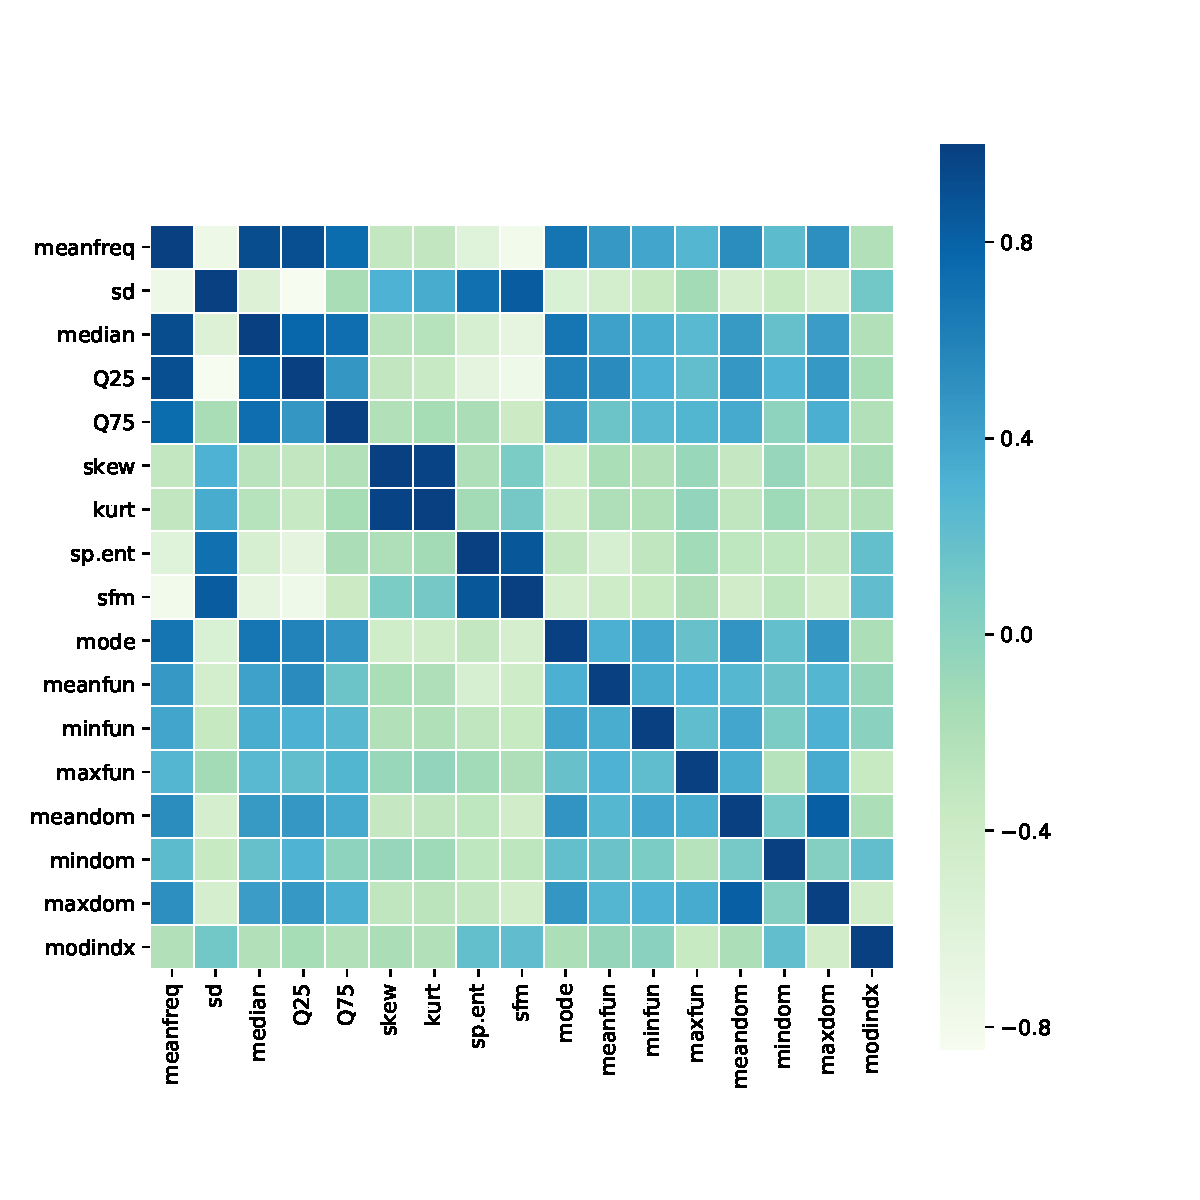
\includegraphics[width=\BoxPlotFigWidth]{figures/correlation_matrix.pdf}}
\begin{figure}[htb]
	\centering
	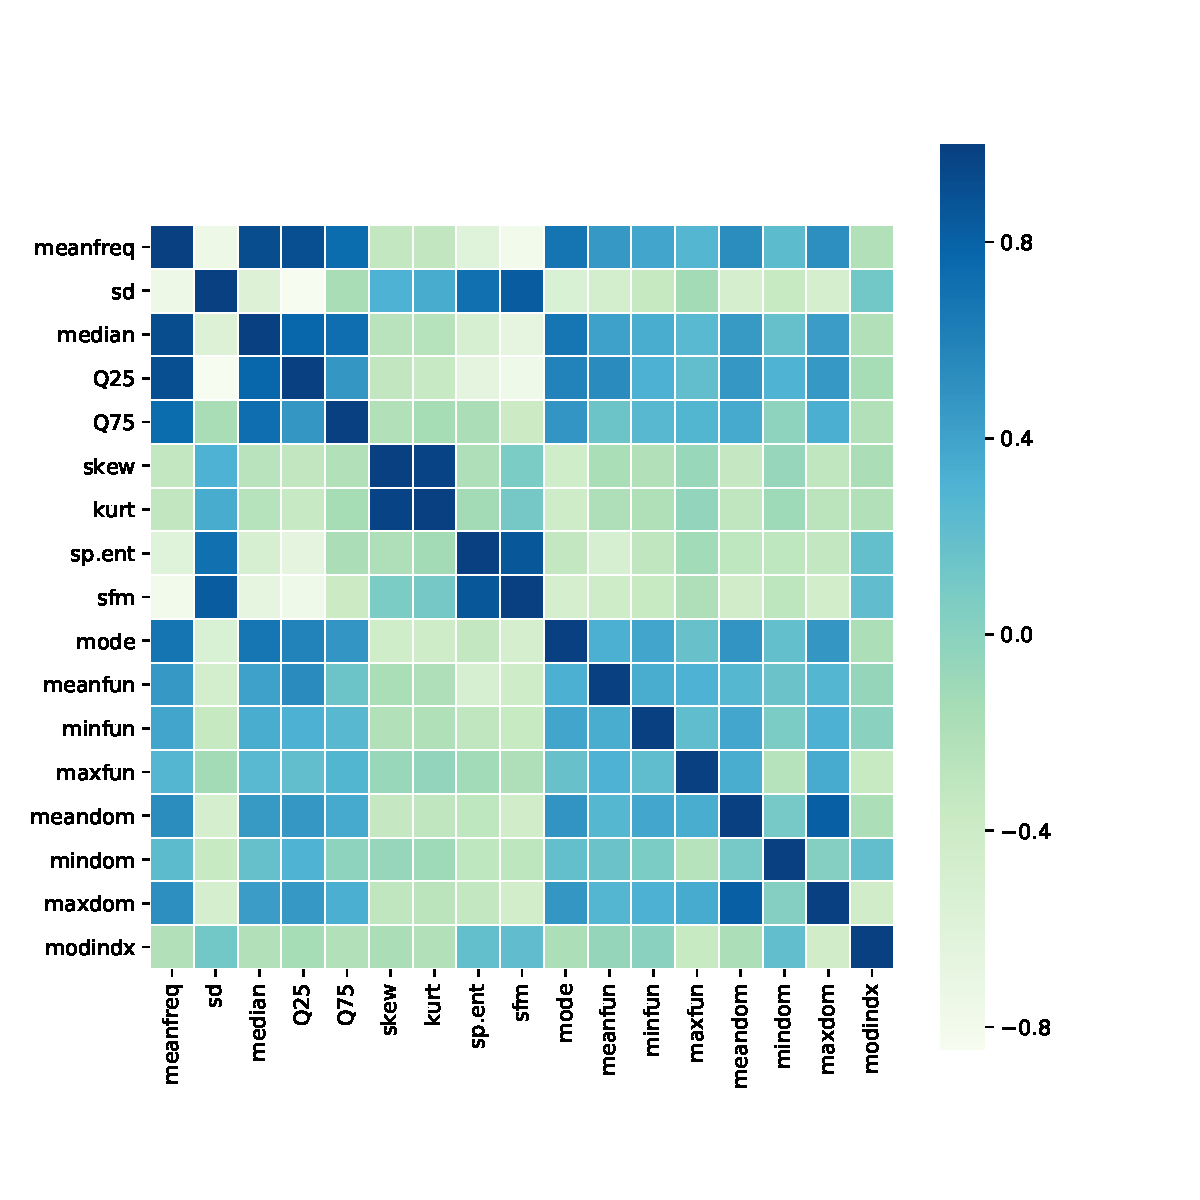
\includegraphics[height=\BoxPlotFigHeight]{figures/correlation_matrix.pdf}
	\caption{Correlation matrix of the dataset.}
	\label{fig_corr_matrix}
\end{figure}
%%%%%%%%%%%% END OF FIGURE %%%%%%%%%%%
%%%%%%%%%%%% FIGURE %%%%%%%%%%%
\setlength{\BoxPlotFigWidth}{0.48\textwidth}
\settoheight{\BoxPlotFigHeight}{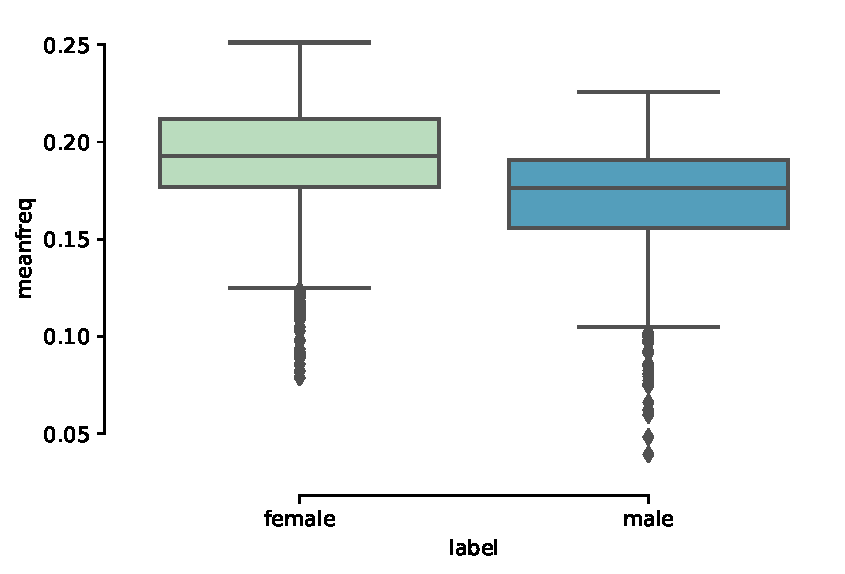
\includegraphics[width=\BoxPlotFigWidth]{figures/meanfreq_boxplot.pdf}}
\begin{figure}[htb]
	% Maximum length
	\hfill%
	\subcaptionbox{\label{fig_meanfreq_box}}{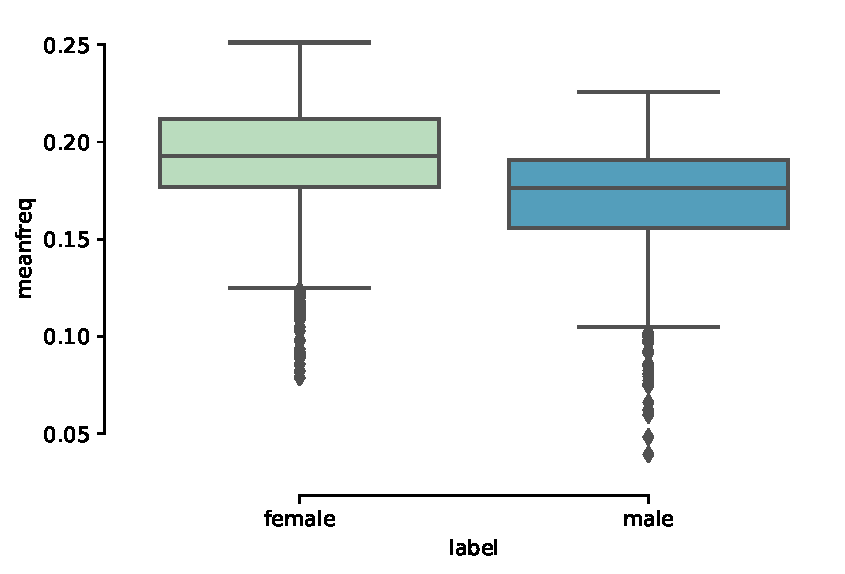
\includegraphics[height=\BoxPlotFigHeight]{figures/meanfreq_boxplot.pdf}}\hfill%
	\subcaptionbox{\label{fig_meanfun_box}}{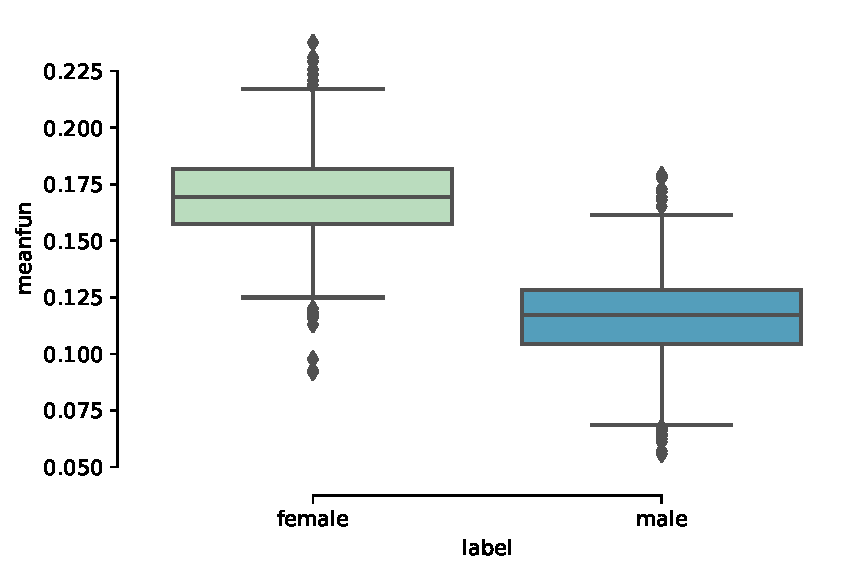
\includegraphics[height=\BoxPlotFigHeight]{figures/meanfun_boxplot.pdf}}\hfill\null%
	\caption{Box plots for (a)-``meanfreq'' and (b)-``meanfun'' features.}
	\label{fig_mean_freq}
\end{figure}
%%%%%%%%%%%% END OF FIGURE %%%%%%%%%%%

In the state-of-the-art, it appears that the fundamental frequency is a key feature for AGR, as stated in Chapter~\ref{chap:introduction}. Intuitively, we also think that the mean frequency should be a good classifier. In order to analyze this, Figs.~\ref{fig_meanfreq_box} and~\ref{fig_meanfun_box} represent the box plots of ``meanfreq'' and ``meanfun'' respectively. 
It can be noticed that ``meanfun'' is indeed a key feature for classification since the overlap between male and female is very low. Regarding ``meanfreq'', the overlap is bigger than for ``meanfun'' but remains rather low. 

Figs.~\ref{fig_meanfreq_facet} and~\ref{fig_meanfun_facet} represent the distribution of male and female with respect to ``meanfreq'' and ``meanfun'' respectively. They confirm the analysis made with the box plot, \ie{} that ``meanfun'' is a key component in AGR and is a far better classifier than ``meanfreq''.
%%%%%%%%%%%% FIGURE %%%%%%%%%%%
\settoheight{\BoxPlotFigHeight}{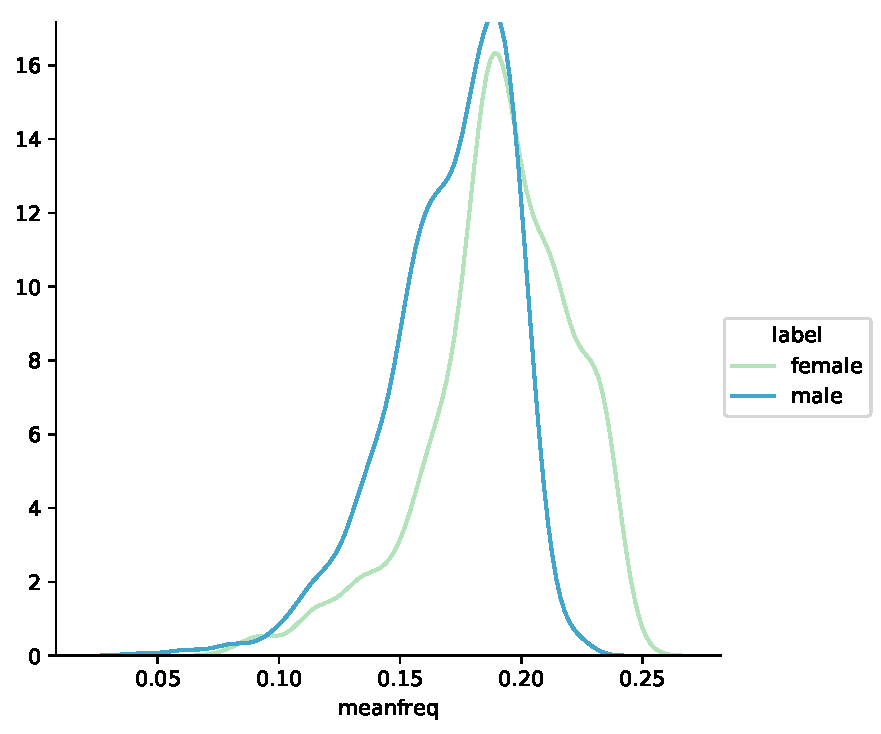
\includegraphics[width=\BoxPlotFigWidth]{figures/meanfreq_facetgrid.pdf}}
\begin{figure}[htb]
	% Maximum length
	\hfill%
	\subcaptionbox{\label{fig_meanfreq_facet}}{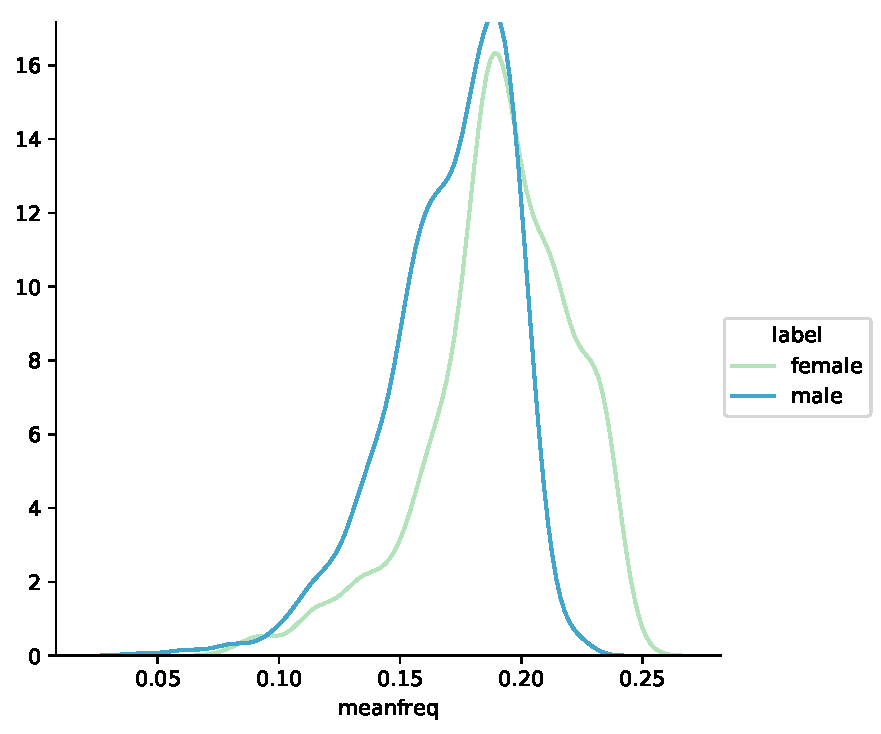
\includegraphics[height=\BoxPlotFigHeight]{figures/meanfreq_facetgrid.pdf}}\hfill%
	\subcaptionbox{\label{fig_meanfun_facet}}{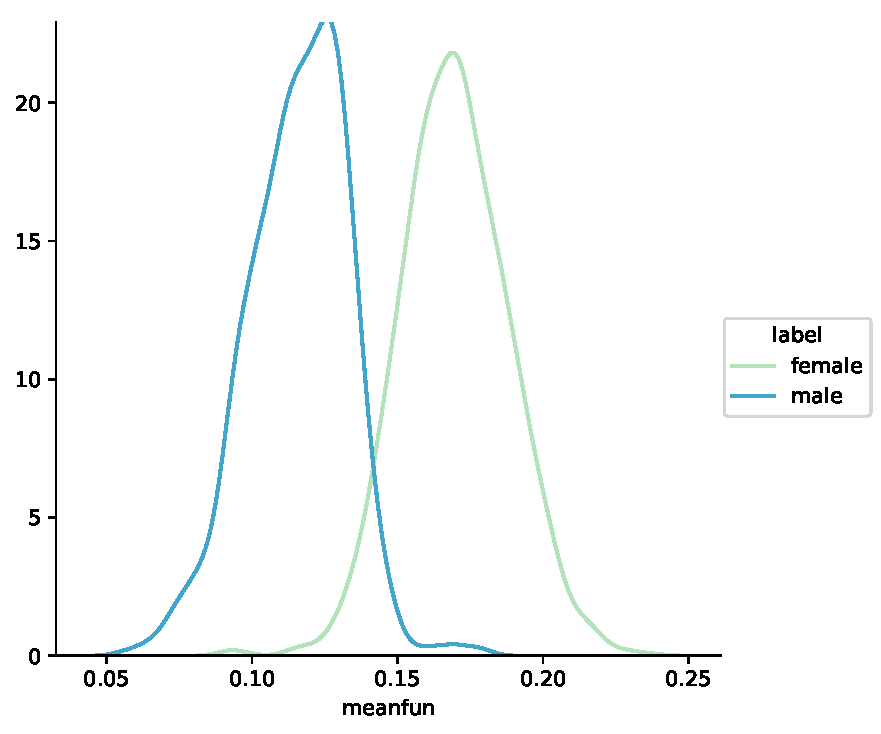
\includegraphics[height=\BoxPlotFigHeight]{figures/meanfun_facetgrid.pdf}}\hfill\null%
	\caption{Distribution of ``male'' and ``female'' for (a)-``meanfreq'' and (b)-``meanfun'' features.}
	\label{fig_facet}
\end{figure}
%%%%%%%%%%%% END OF FIGURE %%%%%%%%%%%


\chapter{Evaluation of the Best Classification Method}
\label{chapter_classification}
\section{Considered classification methods}
\label{sec_considered_classif}

\section{Classification based on the fundamental frequency}
\label{sec_intuitive_approach}
Based on the exploratory data analysis described in Chapter~\ref{chapter_data_exploration}, we propose to perform the classification based on the ``meanfun'' feature alone. 
This will give a baseline for further analysis described in the remaining of this Chapter.

To perform the analysis, we randomly split the dataset into a training set~( \SI{80}{\percent}) and a test set~(\SI{20}{\percent}). The training set is used to fit the models and for best parameter selection if needed. The test set is used to compute the classification error and to compare the models. The classification error considered in the study is the $0-1$ loss.
 
\section{The naive strategy}
\label{sec_naive_strat}
\subsection{Description}
\subsection{Results}
\begin{table}[htb]
	\ra{1.2}
	\caption{Classification Error of the Methods for Different Seed Numbers}
	\begin{center}
		\begin{tabular}{@{} c c c  c c c c @{}}\toprule
			\multirow{2}{*}{Type} & \multirow{2}{*}{Methods} &  \multicolumn{5}{c}{Seed number}\\
			& & 1 & 2 & 3 & 4 & 5 \\
			\midrule
			\multirow{5}{*}{Max. Likelihood} & Logistic reg. & \num{0.0158} & \num{0.0347} & \num{0.0315} & \num{0.0237} & \num{0.0221} \\
			& Logistic reg. - Ridge & \num{0.0158} & \num{0.0315} & \num{0.0315} & \num{0.0189} & \num{0.0284} \\
			& Logistic reg. - Lasso & \num{0.0315} & \num{0.0363} & \num{0.0379} & \num{0.0284} & \num{0.0300} \\
			& LDA & \num{0.0315} & \num{0.0410} & \num{0.0379} & \num{0.0284} & \num{0.0268} \\
			& QDA & \num{0.0347} & \num{0.0347} & \num{0.0347} & \num{0.0268} & \num{0.0363} \\
			\cmidrule{1-7}
			\multirow{5}{*}{Trees} & Tree & \num{0.0379} & \num{0.0426} & \num{0.0315} & \num{0.0284} & \num{0.0300}\\
			& Pruned Tree & \num{0.0394} & \num{0.0473} & \num{0.0347} & \num{0.0363} & \num{0.0300}\\  
			& Bagging & \num{0.0237} & \num{0.0410} & \num{0.0142} & \textbf{\num{0.0174}} & \num{0.0284}\\
			& Random Forest & \num{0.0189} & \num{0.0347} & \textbf{\num{0.0126}} & \num{0.0205} & \num{0.0205}\\
			& XGBoost & \num{0.0189} & \textbf{\num{0.0268}} & \textbf{\num{0.0126}} & \num{0.0205} & \textbf{\num{0.0189}}\\
			\cmidrule{1-7}
			\multirow{2}{*}{SVM} & Linear & \textbf{\num{0.0142}} & \num{0.0315} & \num{0.0284} & \num{0.0189} & \num{0.0252}\\
			& Gaussian & \num{0.0205} & \num{0.0284} & \num{0.0126} & \num{0.0189} & \num{0.0221}\\
			\cmidrule{1-7}
			x & kNN & \num{0.0300} & \num{0.0347} & \num{0.0252} & \num{0.0379} & \num{0.0300}\\
			\bottomrule
			\end{tabular}
			\end{center}
			\label{tab_res_naive}
\end{table}

\begin{table}[htb]
	\ra{1.2}
	\caption{Classification Error of the Methods for Different Seed Numbers with $50/50$ split}
	\begin{center}
		\begin{tabular}{@{} c c c  c c c c @{}}\toprule
			\multirow{2}{*}{Type} & \multirow{2}{*}{Methods} &  \multicolumn{5}{c}{Seed number}\\
			& & 1 & 2 & 3 & 4 & 5 \\
			\midrule
			\multirow{5}{*}{Max. Likelihood} & Logistic reg. & \num{0.0158} & \num{0.0347} & \num{0.0315} & \num{0.0237} & \num{0.0221} \\
			& Logistic reg. - Ridge & \num{0.0158} & \num{0.0315} & \num{0.0315} & \num{0.0189} & \num{0.0284} \\
			& Logistic reg. - Lasso & \num{0.0315} & \num{0.0363} & \num{0.0379} & \num{0.0284} & \num{0.0300} \\
			& LDA & \num{0.0315} & \num{0.0410} & \num{0.0379} & \num{0.0284} & \num{0.0268} \\
			& QDA & \num{0.0347} & \num{0.0347} & \num{0.0347} & \num{0.0268} & \num{0.0363} \\
			\cmidrule{1-7}
			\multirow{5}{*}{Trees} & Tree & \num{0.0379} & \num{0.0426} & \num{0.0315} & \num{0.0284} & \num{0.0300}\\
			& Pruned Tree & \num{0.0394} & \num{0.0473} & \num{0.0347} & \num{0.0363} & \num{0.0300}\\  
			& Bagging & \num{0.0237} & \num{0.0410} & \num{0.0142} & \textbf{\num{0.0174}} & \num{0.0284}\\
			& Random Forest & \num{0.0189} & \num{0.0347} & \textbf{\num{0.0126}} & \num{0.0205} & \num{0.0205}\\
			& XGBoost & \num{0.0189} & \textbf{\num{0.0268}} & \textbf{\num{0.0126}} & \num{0.0205} & \textbf{\num{0.0189}}\\
			\cmidrule{1-7}
			\multirow{2}{*}{SVM} & Linear & \textbf{\num{0.0142}} & \num{0.0315} & \num{0.0284} & \num{0.0189} & \num{0.0252}\\
			& Gaussian & \num{0.0205} & \num{0.0284} & \num{0.0126} & \num{0.0189} & \num{0.0221}\\
			\cmidrule{1-7}
			x & kNN & \num{0.0300} & \num{0.0347} & \num{0.0252} & \num{0.0379} & \num{0.0300}\\
			\bottomrule
		\end{tabular}
	\end{center}
	\label{tab_res_our_strategy}
\end{table}
%%%%%%%%%%%%%%%%%%%%%%%%%%%%%%%%%%%%%%%%%%%%%%
%%%%% TAIL: Appendix, references
%%%%%%%%%%%%%%%%%%%%%%%%%%%%%%%%%%%%%%%%%%%%%%
\appendix
%%%%%%%%%%%%%%%%%%%%%%%%%%%%%%%%%%%%%%%%%%%%%%%%%%%
% Signal Processing Laboratory (LTS5) - EPFL      %
% LaTeX student report template                   %
% Authors:                                        %
%   D. Perdios – dimitris.perdios@epfl.ch         %
%   A. Besson – adrien.besson@epfl.ch             %
% v0.1 - 22.12.16                                 %
% Typeset configuration: pdfLaTeX + Biber         %
%%%%%%%%%%%%%%%%%%%%%%%%%%%%%%%%%%%%%%%%%%%%%%%%%%%


%\blindmathfalse
%\blinddocument
%%%%%%%%%%%%%%%%%%%%%%%%%%%%%%%%%%%%%%%%%%%%%%%%%%%
% Signal Processing Laboratory (LTS5) - EPFL      %
% LaTeX student report template                   %
% Authors:                                        %
%   D. Perdios – dimitris.perdios@epfl.ch         %
%   A. Besson – adrien.besson@epfl.ch             %
% v0.1 - 22.12.16                                 %
% Typeset configuration: pdfLaTeX + Biber         %
%%%%%%%%%%%%%%%%%%%%%%%%%%%%%%%%%%%%%%%%%%%%%%%%%%%


%\cleardoublepage\phantomsection
%\addcontentsline{toc}{chapter}{\bibname}% Add references to ToC (and bookmarks)
%\printbibliography
\printbibliography[heading=bibintoc]
% Remark: heading=bibintoc adds bib in TOC and bookmarks and seems to provide a \phantomsection like facility for hyperref
%TODO: check more on heading=bibintoc option could be usefull to avoid \cleardoublepage\phantom section with TOC, LOF and LOT

\end{document}
